% TEMPLATE for Usenix papers, specifically to meet requirements of
%  USENIX '05
% originally a template for producing IEEE-format articles using LaTeX.
%   written by Matthew Ward, CS Department, Worcester Polytechnic Institute.
% adapted by David Beazley for his excellent SWIG paper in Proceedings,
%   Tcl 96
% turned into a smartass generic template by De Clarke, with thanks to
%   both the above pioneers
% use at your own risk.  Complaints to /dev/null.
% make it two column with no page numbering, default is 10 point

% Munged by Fred Douglis <douglis@research.att.com> 10/97 to separate
% the .sty file from the LaTeX source template, so that people can
% more easily include the .sty file into an existing document.  Also
% changed to more closely follow the style guidelines as represented
% by the Word sample file. 

% Note that since 2010, USENIX does not require endnotes. If you want
% foot of page notes, don't include the endnotes package in the 
% usepackage command, below.

\documentclass[letterpaper,twocolumn,10pt]{article}
\usepackage{usenix,epsfig,endnotes}
\usepackage{algpseudocode}
\usepackage{graphicx}
\usepackage{amsmath}
\usepackage{url}

% \fontfamily{cmr}\selectfont
\begin{document}

%don't want date printed
\date{}

%make title bold and 14 pt font (Latex default is non-bold, 16 pt)
\title{\Large \bf Finding Kernels in Non-Linear Data-Driven CHC Solving}

\author{
{\rm Michael Eden}\\
Trustable Programming \\
Georgia Institute of Technology
}

\maketitle

% Use the following at camera-ready time to suppress page numbers.
% Comment it out when you first submit the paper for review.
% \thispagestyle{empty}


\subsection*{Abstract}

Program verification has seen a lot of progress, but its still unable to
automatically find proofs for industry programs. This paper builds on
data-driven approaches from previous work \cite{data-driven} to provide a
more robust automatic prover for programs with non-linear loop invariants.
It does so by attempting to find the correct kernel for the relation that makes
the invariant linear. This is an easy addition to existing systems and can be
used with any data-driven approach, allowing it to be easily implemented on top
of them. By finding a suitable kernel, many difficult non-linear invariants are
easily found.

\section{Background}

Questions on computability and decidability have perplexed theoretical computer
scientists for many years. Early research showed that some classes of problems
are undecidable, i.e. no algorithm could determine an answer in a finite amount
of time​ \cite{turing}​. However there are incredibly useful problems that fall
into this class,
such as determining if an algorithm will ever end or determining if it contains
errors. Since malicious actors exploit software by finding errors in its code, the
process of automatically finding those errors becomes invaluable to people,
businesses, and the government. There are some who believe that, since the
problem is impossible, it’s not worth pursuing, but only a few years after being
ruled out a solution was discovered and published​ \cite{turing}​.
These two discoveries
weren't conflicting, rather the solution simply didn’t work in all cases.

Even though it was incomplete, that first solution began a mission to find
an ever more (but not quite) complete method. The focus of safety verification
has been to ​attempt to determine if some programs could reach any error states
and not to develop a system that works for all programs \cite{program-termination}.
When rephrased like
this the search seems more optimistic. After all, humans can do this task in a
finite amount of time for many programs. Many systems have been proposed, but
currently encoding programs into a system of Horn Clauses (a special form of
logical equation) stands out \cite{solving-horn-inter}.
If such a system has no solution, then there
is no way for a program to reach an error state. This method has had significant
success but is incomplete in an important way. One of it’s vital tasks is being able
to summarize a loop body so it can avoid essentially simulating a run of the input
program. This is an impossible task, one basically has to find a function that maps
every iteration of a loop to a program state efficiently. A common problem is that
this function becomes too specific, i.e. it becomes a table of previous iterations
and their states. Such a table is not amenable to generalization or abstraction; it
is too specific to past iterations to help understand future ones. Specifically, the
problem described here is the issue of finding weaker interpolants when finding
loop invariants.


This research focuses on finding more general (weaker) loop invariants in
the realm of boolean and integer arithmetic.
Data is collected from past papers and researchers to see which programs were
difficult to solve and to inform heuristics developed in this work.
Since this is focused on non-linear problems and is meant to augment existing
linear solvers, this method is limited by SMT solver used (Z3 in this case).
Hopefully these weaker non-linear interpolants will generalize better to the
rest of state space.

\section{Related Work}

In 1936 Alan Turing proved that no algorithm could determine if a program will
always terminate or continue to run forever using a finite amount of time
\cite{turing}.
Unfortunately this also means that many related and useful questions are also
undecidable about general programs. For instance one cannot always know whether
a program will have errors in it until it’s actually run, an obvious property
of interest in industry. Still thirteen years later Turing also published a now
widely used method of proving program termination \cite{turing}.
In the face of a provably impossible problem, Turing’s method simply never halts
when it cannot decide on an answer.

This led to the comparatively easier problem of answering ``Will Halt'', ``Will
Not Halt'' and ``Unknown'' for every program.
Since then the fields of program termination, software verification,
program equivalence, etc. have all been attempting to slim down the cases in
which their algorithms result in ``Unknown''
\cite{program-termination} \cite{harris} \cite{do-good}.
A driving and practical motivation for program verification is that software
is embedded into the United States' electric grid, medical instruments,
nuclear weapons storage, and other vital components of infrastructure.
Proving that these systems work correctly is both beneficial at face
value and prevent attackers from compromising them.

Verification has thankfully seen a lot of progress since it was able to transform
programs into a concise logical representation known as Horn Clauses and then
solve the resulting systems efficiently ​\cite{solving-horn-inter}.
As reported by Albarghouthi, there is now a fission in the
approach used to solve these systems ​\cite{under-over-approx}.
One style attempts to find properties at every point in the program while the
other only tries to find properties when they are needed to prove some goal
\cite{under-over-approx}.
It might seem that the former is clearly worse, however it can
solve some programs which the latter cannot and vice-versa.
The disagreement here, at its core, is about finding the right property to
prove. A lot of research effort has been poured into this problem, and so far
the consensus is leaning towards the latter ``lazy'' approach
\cite{under-over-approx} \cite{solving-horn-inter} \cite{lazy-interpolants}.

A quick consequence of the ``lazy'' approach is the ability to completely
automate the proving process. A key in the fully automated verification process
is the ability to find some invariant that is consistent across every iteration
of a loop. Since programs without loops (and without recursion) are relatively
simple, it is this automatic finding of loop invariants that has taken hold of
a lot of research today \cite{solving-horn-inter} \cite{harris}.
Issues with finding these invariants are consistent with the overall theme
and difficulty of finding the right property to prove.
In McMillan’s research, he demonstrates an automatic proof that a loop starting
at zero and incrementing a counter by two can never be forty-one
\cite{solving-horn-inter}.

\begin{figure}[h]
\begin{algorithmic}
\Function{count}{$N$}
\State $i \gets 0$
\While{$i < N$}
  \State $i \gets i + 2$
\EndWhile
\State \textbf{assert} $i \neq 41$
\EndFunction
\end{algorithmic}
\caption{Program described in \cite{solving-horn-inter}}
\end{figure}

However this method does not prove ``the loop starts at an even number and adds
an even number, so it cannot be odd'' as many people might hope.
Instead it shows ``once the loop gets to 40, the only next possible value is
42'' \cite{solving-horn-inter}.
If one tries to ask the analyzer to show that the loop will always be even,
it cannot. It tends to generate facts that are too specific, large, and complex
about the current program state and does not provide a more general and useful fact​
\cite{beautiful-interpolants} \cite{interpolant-strength}.
According to Albarghouthi, the principle of Occam’s Razor should somehow be
embedded into the invariant finding process in the hopes a simpler fact will be
a more useful one. This is akin to ``regularization'' in many statistical methods.

Albarghouthi has made significant progress in finding incredibly concise and
general interpolants (a precursor to loop invariants) in Quantifier Free Linear
Rational Arithmetic (QFLRA). This encompasses a significant but not total
portion of programs in industry \cite{beautiful-interpolants}. Finding these
loop invariants are vital since they are the biggest roadblock to automatic
verification. Automatic is important here since most use cases involve large
complex software that would take a long time to annotate with invariants.

Another gap in the current research is the availability of a dataset of real-world
programs. Many of the seminal papers here are from Microsoft Research, which tests
their methods on Windows Drivers ​\cite{do-good}.
This research benefits from the existing set of testable programs but, being a
data-driven approach, will always benefit more from more data.
Hopefully there will be a large de-facto dataset in the future, since this is a
major hurdle when quantifying new methods and improving old ones.

\section{Implementation}

The implementation of this method is based off the idea that \cite{data-driven}
does a great job with linear data and that it can be extended to fit non-linear
data by simply applying a different kernel. The kernel can be ``guessed'' by
analyzing the source code of the incoming program. In the method described in
\cite{data-driven} there was no direct analysis of the program source, so
process would be more difficult. It's also possible to learn the correct space
purely through the data, but this takes a large amount of it.
Solving logical systems, therefore, have a strange relationship with statistical
methods since they contain very little data and demand a perfect fit (completely
``over-fitted''). As described earlier a ``simpler'' solution is preferable so
that it can generalize, but this generalization must not cause any loss in
accuracy.

\subsection{Linear CHCs}

The function described in Figure \ref{fig:quadratic} is a simple quadratic
relationship between $x$ and  $y$. One might thing that this non-linearity
would pose a problem, but that's not the case.

\begin{figure}[h]
\begin{algorithmic}
\Function{quadratic}{}
\State $x \gets 1, y \gets 1$
\Loop
  \State $y \gets y + x$
  \State $x \gets x + 2$
\State \textbf{assert} $y \geq x$
\EndLoop
\EndFunction
\end{algorithmic}
\caption{Simple quadratic program}
\label{fig:quadratic}
\end{figure}

However a linear decision boundary is quickly found using the method described
in \cite{data-driven}, the classifier found three linear boundaries tied
together by a decision tree.

\begin{figure}[h]
  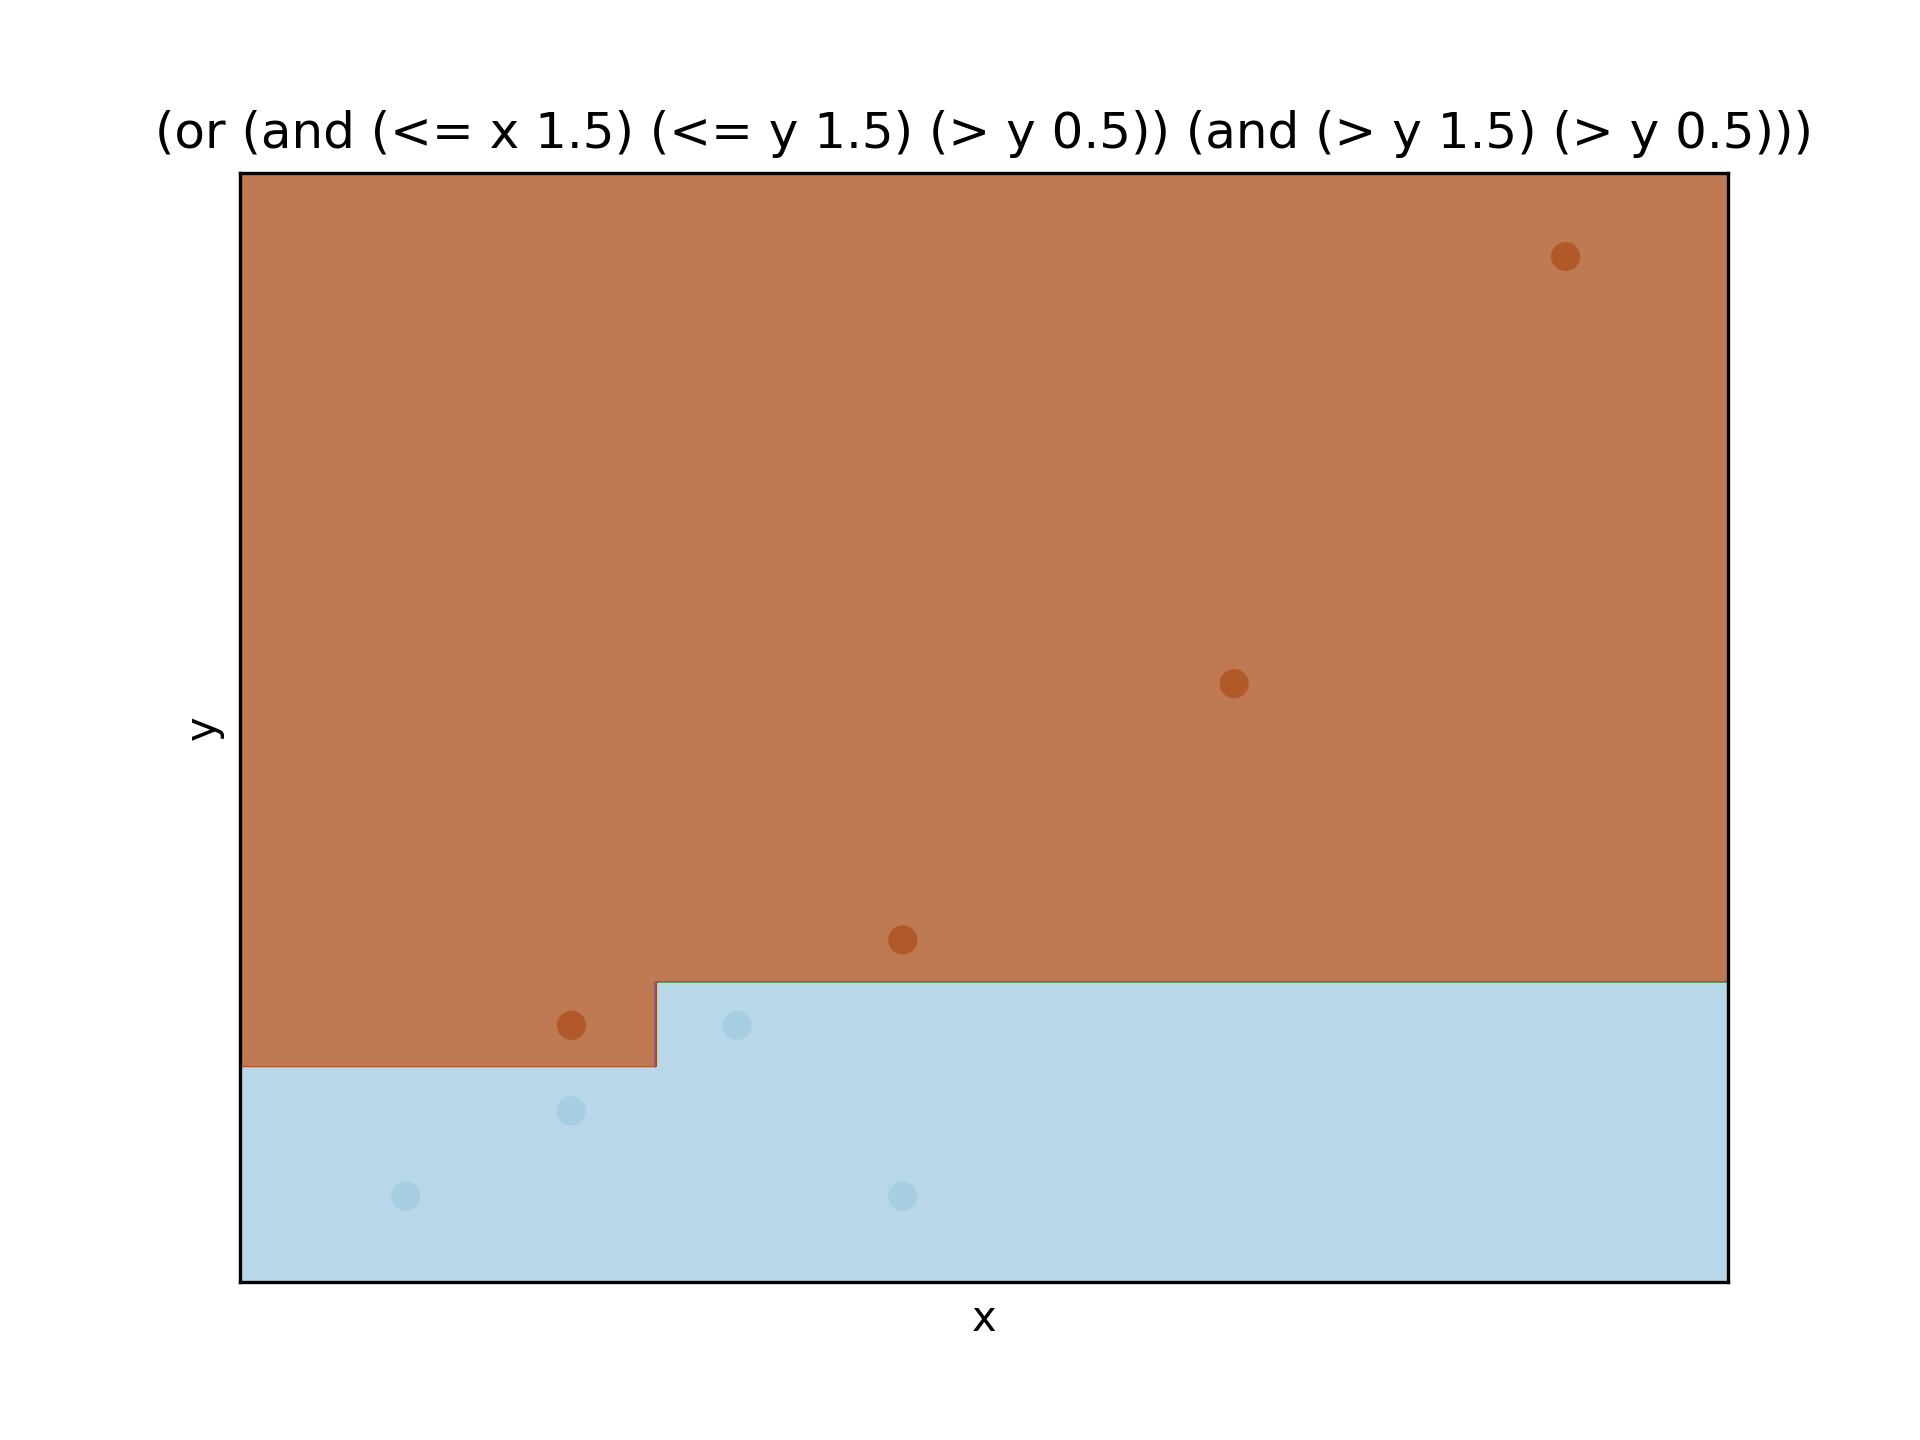
\includegraphics[width=0.5\textwidth]{quadratic}
  \caption{Decision boundary created by Figure \ref{fig:quadratic}}
  \label{fig:quadratic-graph}
\end{figure}

Figure \ref{fig:quadratic-graph} shows the output
of the tool developed for this project on the program in Figure
\ref{fig:quadratic}. It's title is the decision boundary encoded into Z3's
s-expressions, a necessary step in the process, it is the equivalent of:

$$
(x \leq 1.5 \land 0.5 < y \leq 1.5) \lor (y > 1.5 > 0.5)
$$

The iteration is simple, positive (brown red) and negative (blue) points are
loaded into a classifier to be separated. Positive points are simply variables
values that the program will encounter (found by unfolding the loop) and that
agree with the goal (if they do not, one can show the goal is wrong).
A classifier is built and it's function is assigned to the loop invariant in Z3.
If the classifier finds an invariant strong enough to prove the goal, Z3 stops
and the process completes. If the invariant is too weak, Z3 finds a
counterexample which then gets added to the pool of negative points and the
process restarts. To bootstrap the first negative point,
\texttt{true} or the goal function is used as the initial invariant.
So far this tool has only emulated \cite{data-driven} but it will soon be
extended  to do more. Source code is freely available online \cite{github}.

Naturally, this depends on Z3's ability to produce counterexamples, which means
Z3's limited ability to handle transcendental functions ($e^x$, $\sin x$, $x!$,
etc.) also applies here, limiting the scope to polynomials.

\subsection{Non-Linear CHCs}

Writing a simple recurrence containing a multiplication (Figure \ref{fig:cubic})
grinds the previous method to a halt.

\begin{figure}[h]
\begin{algorithmic}
\Function{cubic}{}
\State $x \gets 1, y \gets 1, z \gets 1$
\Loop
  \State $x \gets x + z^2$
  \State $y \gets y + z^2 - 2z$
  \State $z \gets z + 1$
\State \textbf{assert} $G(x, y, z)$
\EndLoop
\EndFunction
\end{algorithmic}
\caption{Slightly more complex program}
\label{fig:cubic}
\end{figure}

Solving the recurrence $g(n) = g(n) + n^2$ and $g(n) = g(n) + n^2 - 2n$ shows us
that both $x$ and $y$ are functions of degree three.
However it might not always be easy to solve recurrences directly, instead it is
easier to approximate the degree and attempt to classify the points in a higher
space. This is where picking the correct space becomes crucial, too large and
sparse and it will take too long to traverse, too small and it won't be
expressive enough.

The degree isn't solely decided by the program either, the goal $G(x, y, z)$ is
also relevant. For instance if Figure \ref{fig:cubic} contained

$$
G(x, y, z) = x \geq y
$$

then a simple linear boundary would suffice. However if the goal was more
complex like

$$
G(x, y, z) = y + z^2 \geq x
$$

then linear boundaries won't do, and the method in \cite{data-driven} iterates
forever generating lines that approximate a parabola.
It seems that $x$ and $y$ are of close enough degree to each other and $z$ is
far away from both. By analyzing the source we can tell the maximum degree these
variables might become:

$$
z: 1,~~~~ y: 1 + 2(z) = 3,~~~ x: 1 + 2(z) = 3, 
$$

Further we can look at all the possible ways each term is used (1), or simply
take each variable to its maximum degree (2), or look the goals terms (3):

\begin{align}
  T &= \{x, y, z, z^2\} \\
  P &= \{x^1, x^2, x^3, y^1, y^2, y^3, z^1\} \\
  Q &= \{x, y, z^2\}
\end{align}

For the quadratic $G$ itself is enough to act as the invariant, meaning space
$Q$ is the optimal space to search through. The general solution to the
recurrence, however, would not be covered by $Q$:

$$
x = y + z^2 - z ~~\land~~ z > 0
$$

Since this is the ground truth for the loop invariant, we'd like all classifiers
to look through no space larger than this.


\section{Experiments}

% different spaces
% polynomial kernel svm taking a long time
% simple = good

A tool was made to test different heuristics when evaluating these non-linear
programs \cite{github}. It analyzes the source and pulls out terms such as $T$,
$P$, and $Q$, adding them to the dataset and trying to classify them.
A large dataset of positive and negative points was also used from the
indefinitely-iterating purely linear method. When these points where classified
with added dimensions they were clearly linearly separable. However simply using
a polynomial SVM with a decision tree took hours to complete on a test machine.

The most successful heuristic ended up being $Q$, or terms only in the goal,
since the goal has to be somehow expressed within the invariant. Using a simple
linear SVM was much faster than the polynomial SVM (a few milliseconds for 1000
data points) so the best strategy so far is to attempt to fit many different
combinations of degrees in parallel. Since the number of data points is usually
small, given a max degree of $\Delta$ and number of variables $n$ that would
generate:

$$
\text{number of classifiers} = 2^{n\Delta}
$$

The example above would train $2^9 = 512$ linear SVMs, which is a lot, but since
\texttt{scikit-learn}'s SVM is so fast it can generally be done rather quickly.
Further if the list of term combinations is ordered with more likely sets first
(such as $Q$), it will likely find a separable line quicker.

\section{Conclusion}

Overall finding non-linear invariants is harder, but not so much harder than
linear invariants. On the other hand even simple exponential functions will
cause Z3 to give ``unknown''.
This method is a simple addition to many data-driven methods that can make a lot
of programs that users expect to be solvable actually solvable. What this and
many other methods need is a larger and more standard data set to learn from.
Future work to aid this automatic verification would definitely include manually
collecting large data-sets from important open source projects.
Another important addition to this work would be to add it to a layer in SeaHorn
so that it could be used in production with any LLVM language.

\vfill

\pagebreak

{
\footnotesize
\bibliographystyle{acm}
\bibliography{sample}
}


% \theendnotes

\end{document}







